% Options for packages loaded elsewhere
% Options for packages loaded elsewhere
\PassOptionsToPackage{unicode}{hyperref}
\PassOptionsToPackage{hyphens}{url}
\PassOptionsToPackage{dvipsnames,svgnames,x11names}{xcolor}
%
\documentclass[
  letterpaper,
  DIV=11,
  numbers=noendperiod]{scrartcl}
\usepackage{xcolor}
\usepackage{amsmath,amssymb}
\setcounter{secnumdepth}{-\maxdimen} % remove section numbering
\usepackage{iftex}
\ifPDFTeX
  \usepackage[T1]{fontenc}
  \usepackage[utf8]{inputenc}
  \usepackage{textcomp} % provide euro and other symbols
\else % if luatex or xetex
  \usepackage{unicode-math} % this also loads fontspec
  \defaultfontfeatures{Scale=MatchLowercase}
  \defaultfontfeatures[\rmfamily]{Ligatures=TeX,Scale=1}
\fi
\usepackage{lmodern}
\ifPDFTeX\else
  % xetex/luatex font selection
\fi
% Use upquote if available, for straight quotes in verbatim environments
\IfFileExists{upquote.sty}{\usepackage{upquote}}{}
\IfFileExists{microtype.sty}{% use microtype if available
  \usepackage[]{microtype}
  \UseMicrotypeSet[protrusion]{basicmath} % disable protrusion for tt fonts
}{}
\makeatletter
\@ifundefined{KOMAClassName}{% if non-KOMA class
  \IfFileExists{parskip.sty}{%
    \usepackage{parskip}
  }{% else
    \setlength{\parindent}{0pt}
    \setlength{\parskip}{6pt plus 2pt minus 1pt}}
}{% if KOMA class
  \KOMAoptions{parskip=half}}
\makeatother
% Make \paragraph and \subparagraph free-standing
\makeatletter
\ifx\paragraph\undefined\else
  \let\oldparagraph\paragraph
  \renewcommand{\paragraph}{
    \@ifstar
      \xxxParagraphStar
      \xxxParagraphNoStar
  }
  \newcommand{\xxxParagraphStar}[1]{\oldparagraph*{#1}\mbox{}}
  \newcommand{\xxxParagraphNoStar}[1]{\oldparagraph{#1}\mbox{}}
\fi
\ifx\subparagraph\undefined\else
  \let\oldsubparagraph\subparagraph
  \renewcommand{\subparagraph}{
    \@ifstar
      \xxxSubParagraphStar
      \xxxSubParagraphNoStar
  }
  \newcommand{\xxxSubParagraphStar}[1]{\oldsubparagraph*{#1}\mbox{}}
  \newcommand{\xxxSubParagraphNoStar}[1]{\oldsubparagraph{#1}\mbox{}}
\fi
\makeatother

\usepackage{color}
\usepackage{fancyvrb}
\newcommand{\VerbBar}{|}
\newcommand{\VERB}{\Verb[commandchars=\\\{\}]}
\DefineVerbatimEnvironment{Highlighting}{Verbatim}{commandchars=\\\{\}}
% Add ',fontsize=\small' for more characters per line
\usepackage{framed}
\definecolor{shadecolor}{RGB}{241,243,245}
\newenvironment{Shaded}{\begin{snugshade}}{\end{snugshade}}
\newcommand{\AlertTok}[1]{\textcolor[rgb]{0.68,0.00,0.00}{#1}}
\newcommand{\AnnotationTok}[1]{\textcolor[rgb]{0.37,0.37,0.37}{#1}}
\newcommand{\AttributeTok}[1]{\textcolor[rgb]{0.40,0.45,0.13}{#1}}
\newcommand{\BaseNTok}[1]{\textcolor[rgb]{0.68,0.00,0.00}{#1}}
\newcommand{\BuiltInTok}[1]{\textcolor[rgb]{0.00,0.23,0.31}{#1}}
\newcommand{\CharTok}[1]{\textcolor[rgb]{0.13,0.47,0.30}{#1}}
\newcommand{\CommentTok}[1]{\textcolor[rgb]{0.37,0.37,0.37}{#1}}
\newcommand{\CommentVarTok}[1]{\textcolor[rgb]{0.37,0.37,0.37}{\textit{#1}}}
\newcommand{\ConstantTok}[1]{\textcolor[rgb]{0.56,0.35,0.01}{#1}}
\newcommand{\ControlFlowTok}[1]{\textcolor[rgb]{0.00,0.23,0.31}{\textbf{#1}}}
\newcommand{\DataTypeTok}[1]{\textcolor[rgb]{0.68,0.00,0.00}{#1}}
\newcommand{\DecValTok}[1]{\textcolor[rgb]{0.68,0.00,0.00}{#1}}
\newcommand{\DocumentationTok}[1]{\textcolor[rgb]{0.37,0.37,0.37}{\textit{#1}}}
\newcommand{\ErrorTok}[1]{\textcolor[rgb]{0.68,0.00,0.00}{#1}}
\newcommand{\ExtensionTok}[1]{\textcolor[rgb]{0.00,0.23,0.31}{#1}}
\newcommand{\FloatTok}[1]{\textcolor[rgb]{0.68,0.00,0.00}{#1}}
\newcommand{\FunctionTok}[1]{\textcolor[rgb]{0.28,0.35,0.67}{#1}}
\newcommand{\ImportTok}[1]{\textcolor[rgb]{0.00,0.46,0.62}{#1}}
\newcommand{\InformationTok}[1]{\textcolor[rgb]{0.37,0.37,0.37}{#1}}
\newcommand{\KeywordTok}[1]{\textcolor[rgb]{0.00,0.23,0.31}{\textbf{#1}}}
\newcommand{\NormalTok}[1]{\textcolor[rgb]{0.00,0.23,0.31}{#1}}
\newcommand{\OperatorTok}[1]{\textcolor[rgb]{0.37,0.37,0.37}{#1}}
\newcommand{\OtherTok}[1]{\textcolor[rgb]{0.00,0.23,0.31}{#1}}
\newcommand{\PreprocessorTok}[1]{\textcolor[rgb]{0.68,0.00,0.00}{#1}}
\newcommand{\RegionMarkerTok}[1]{\textcolor[rgb]{0.00,0.23,0.31}{#1}}
\newcommand{\SpecialCharTok}[1]{\textcolor[rgb]{0.37,0.37,0.37}{#1}}
\newcommand{\SpecialStringTok}[1]{\textcolor[rgb]{0.13,0.47,0.30}{#1}}
\newcommand{\StringTok}[1]{\textcolor[rgb]{0.13,0.47,0.30}{#1}}
\newcommand{\VariableTok}[1]{\textcolor[rgb]{0.07,0.07,0.07}{#1}}
\newcommand{\VerbatimStringTok}[1]{\textcolor[rgb]{0.13,0.47,0.30}{#1}}
\newcommand{\WarningTok}[1]{\textcolor[rgb]{0.37,0.37,0.37}{\textit{#1}}}

\usepackage{longtable,booktabs,array}
\newcounter{none} % for unnumbered tables
\usepackage{calc} % for calculating minipage widths
% Correct order of tables after \paragraph or \subparagraph
\usepackage{etoolbox}
\makeatletter
\patchcmd\longtable{\par}{\if@noskipsec\mbox{}\fi\par}{}{}
\makeatother
% Allow footnotes in longtable head/foot
\IfFileExists{footnotehyper.sty}{\usepackage{footnotehyper}}{\usepackage{footnote}}
\makesavenoteenv{longtable}
\usepackage{graphicx}
\makeatletter
\newsavebox\pandoc@box
\newcommand*\pandocbounded[1]{% scales image to fit in text height/width
  \sbox\pandoc@box{#1}%
  \Gscale@div\@tempa{\textheight}{\dimexpr\ht\pandoc@box+\dp\pandoc@box\relax}%
  \Gscale@div\@tempb{\linewidth}{\wd\pandoc@box}%
  \ifdim\@tempb\p@<\@tempa\p@\let\@tempa\@tempb\fi% select the smaller of both
  \ifdim\@tempa\p@<\p@\scalebox{\@tempa}{\usebox\pandoc@box}%
  \else\usebox{\pandoc@box}%
  \fi%
}
% Set default figure placement to htbp
\def\fps@figure{htbp}
\makeatother


% definitions for citeproc citations
\NewDocumentCommand\citeproctext{}{}
\NewDocumentCommand\citeproc{mm}{%
  \begingroup\def\citeproctext{#2}\cite{#1}\endgroup}
\makeatletter
 % allow citations to break across lines
 \let\@cite@ofmt\@firstofone
 % avoid brackets around text for \cite:
 \def\@biblabel#1{}
 \def\@cite#1#2{{#1\if@tempswa , #2\fi}}
\makeatother
\newlength{\cslhangindent}
\setlength{\cslhangindent}{1.5em}
\newlength{\csllabelwidth}
\setlength{\csllabelwidth}{3em}
\newenvironment{CSLReferences}[2] % #1 hanging-indent, #2 entry-spacing
 {\begin{list}{}{%
  \setlength{\itemindent}{0pt}
  \setlength{\leftmargin}{0pt}
  \setlength{\parsep}{0pt}
  % turn on hanging indent if param 1 is 1
  \ifodd #1
   \setlength{\leftmargin}{\cslhangindent}
   \setlength{\itemindent}{-1\cslhangindent}
  \fi
  % set entry spacing
  \setlength{\itemsep}{#2\baselineskip}}}
 {\end{list}}
\usepackage{calc}
\newcommand{\CSLBlock}[1]{\hfill\break\parbox[t]{\linewidth}{\strut\ignorespaces#1\strut}}
\newcommand{\CSLLeftMargin}[1]{\parbox[t]{\csllabelwidth}{\strut#1\strut}}
\newcommand{\CSLRightInline}[1]{\parbox[t]{\linewidth - \csllabelwidth}{\strut#1\strut}}
\newcommand{\CSLIndent}[1]{\hspace{\cslhangindent}#1}



\setlength{\emergencystretch}{3em} % prevent overfull lines

\providecommand{\tightlist}{%
  \setlength{\itemsep}{0pt}\setlength{\parskip}{0pt}}



 


\KOMAoption{captions}{tableheading}
\makeatletter
\@ifpackageloaded{caption}{}{\usepackage{caption}}
\AtBeginDocument{%
\ifdefined\contentsname
  \renewcommand*\contentsname{Table of contents}
\else
  \newcommand\contentsname{Table of contents}
\fi
\ifdefined\listfigurename
  \renewcommand*\listfigurename{List of Figures}
\else
  \newcommand\listfigurename{List of Figures}
\fi
\ifdefined\listtablename
  \renewcommand*\listtablename{List of Tables}
\else
  \newcommand\listtablename{List of Tables}
\fi
\ifdefined\figurename
  \renewcommand*\figurename{Figure}
\else
  \newcommand\figurename{Figure}
\fi
\ifdefined\tablename
  \renewcommand*\tablename{Table}
\else
  \newcommand\tablename{Table}
\fi
}
\@ifpackageloaded{float}{}{\usepackage{float}}
\floatstyle{ruled}
\@ifundefined{c@chapter}{\newfloat{codelisting}{h}{lop}}{\newfloat{codelisting}{h}{lop}[chapter]}
\floatname{codelisting}{Listing}
\newcommand*\listoflistings{\listof{codelisting}{List of Listings}}
\makeatother
\makeatletter
\makeatother
\makeatletter
\@ifpackageloaded{caption}{}{\usepackage{caption}}
\@ifpackageloaded{subcaption}{}{\usepackage{subcaption}}
\makeatother
\usepackage{bookmark}
\IfFileExists{xurl.sty}{\usepackage{xurl}}{} % add URL line breaks if available
\urlstyle{same}
\hypersetup{
  pdftitle={Cuckoo Eggs Dimension},
  pdfauthor={Deborah Elesie},
  colorlinks=true,
  linkcolor={blue},
  filecolor={Maroon},
  citecolor={Blue},
  urlcolor={Blue},
  pdfcreator={LaTeX via pandoc}}


\title{Cuckoo Eggs Dimension}
\author{Deborah Elesie}
\date{2026-10-30}
\begin{document}
\maketitle

\renewcommand*\contentsname{Table of contents}
{
\setcounter{tocdepth}{3}
\tableofcontents
}

\subsection{Introduction}\label{introduction}

The Cuckoo bird is known for its unique reproductive strategy: brood
parasitism. Instead of building their own nests, female cuckoos lay
their eggs in the nests of other bird species (the hosts), leaving the
host birds to incubate and raise the cuckoo chicks.

\begin{figure}

\centering{

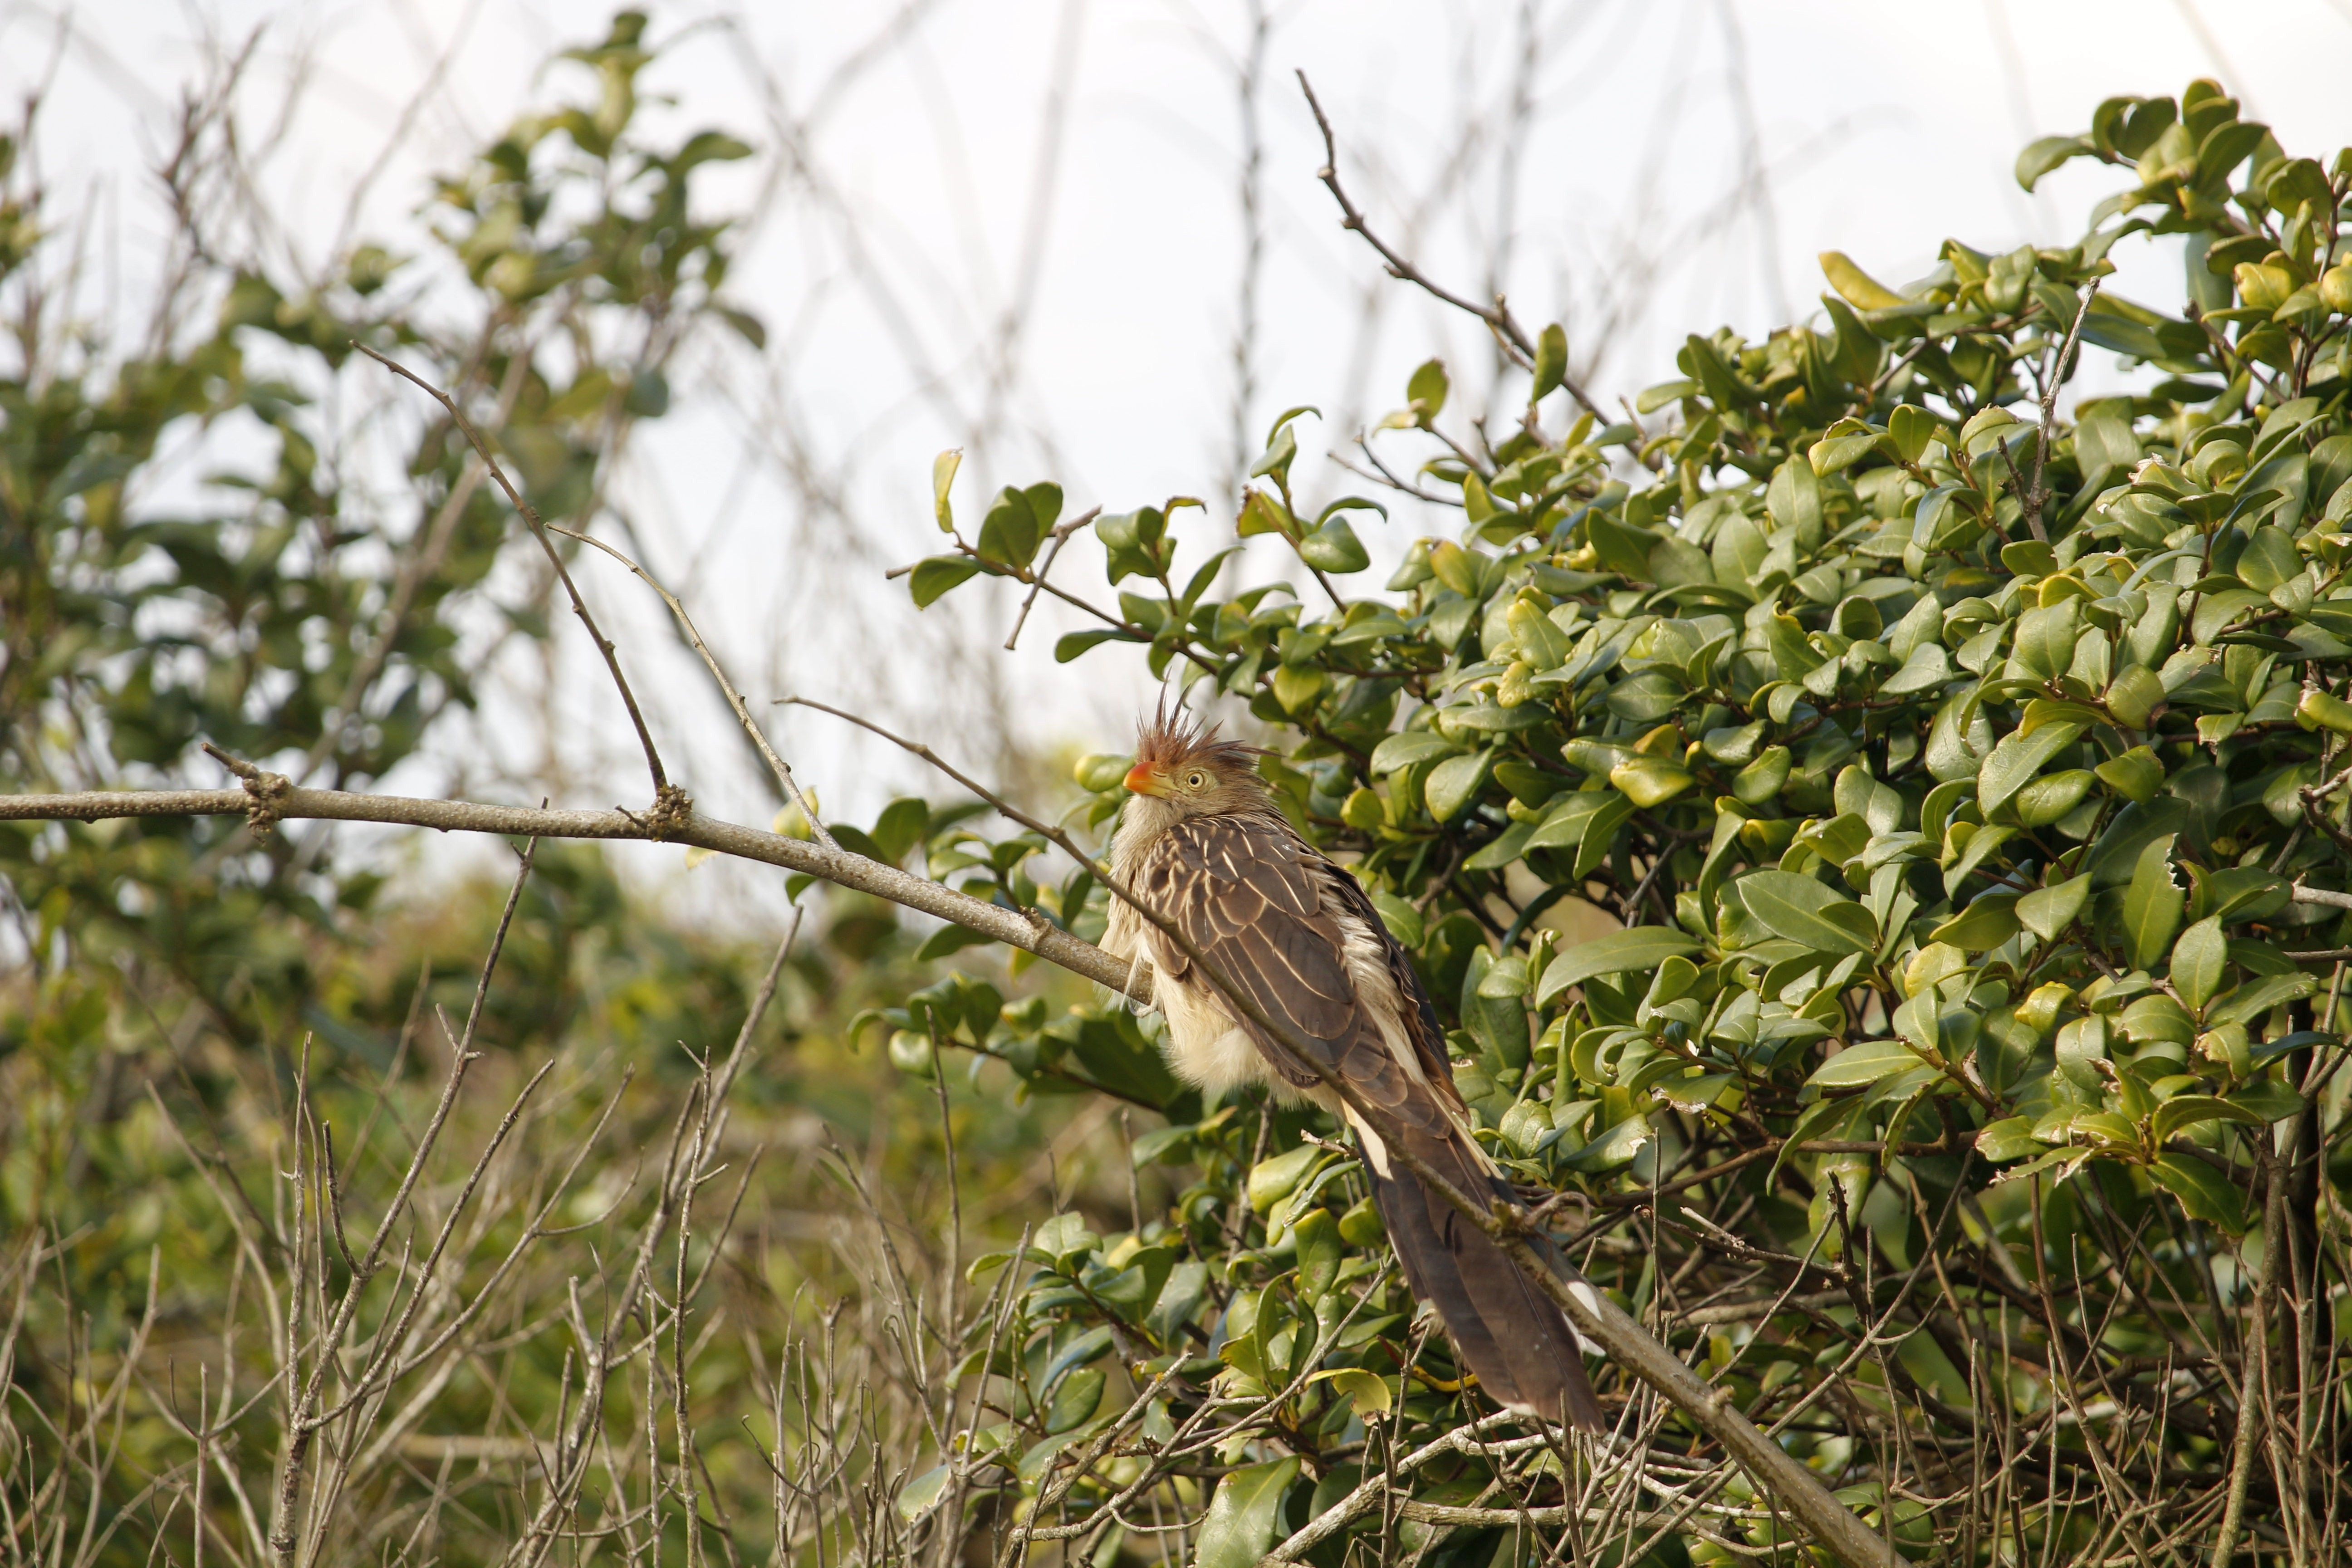
\includegraphics[width=0.5\linewidth,height=\textheight,keepaspectratio]{Capstone_project_files/mediabag/pexels-photo-3860887.jpg}

}

\caption{\label{fig-cuckoobird-image}A picture of Cuckoo bird in the
wild}

\end{figure}%

This report analyzes the physical dimensions of 120 cuckoo eggs found in
the nests of six different host bird species. The dataset, sourced from
the \texttt{DAAG} package (Maindonald et al., 2015), contains
\textbf{three primary variables}: the length of the egg in millimeters,
the breadth of the egg in millimeters, and the species of the host bird.

\subsection{Questions}\label{questions}

For this report, the main objective is to check if there's any
significant difference between the egg sizes across the different host
species. To answer this, we will look at two specific questions:

\begin{enumerate}
\def\labelenumi{\arabic{enumi}.}
\tightlist
\item
  Is there a statistical difference in the \textbf{length} of eggs laid
  by the different bird species?
\item
  Is there a statistical difference in the \textbf{breadth} of eggs laid
  by the different bird species?
\end{enumerate}

\subsection{Data Import and
Inspection}\label{data-import-and-inspection}

Let's start by importing the necessary packages and using basic
inspection functions such as \texttt{head()}, \texttt{tail()}, and
\texttt{str()} to ensure the data was loaded correctly and to understand
its structure.

\begin{Shaded}
\begin{Highlighting}[]
\CommentTok{\# Load packages}
\FunctionTok{library}\NormalTok{(tidyverse)}
\FunctionTok{library}\NormalTok{(janitor)}
\FunctionTok{library}\NormalTok{(car)}

\CommentTok{\# Import data}
\NormalTok{cuckoo\_data }\OtherTok{\textless{}{-}} \FunctionTok{read\_csv}\NormalTok{(}\StringTok{"https://raw.githubusercontent.com/xrander/bootcamp{-}test/master/data/cuckoo.csv"}\NormalTok{) }\SpecialCharTok{|\textgreater{}} 
\NormalTok{  janitor}\SpecialCharTok{::}\FunctionTok{clean\_names}\NormalTok{()}

\CommentTok{\# Inspect data}
\FunctionTok{head}\NormalTok{(cuckoo\_data, }\DecValTok{20}\NormalTok{)}
\end{Highlighting}
\end{Shaded}

\begin{verbatim}
# A tibble: 20 x 3
   length breadth species     
    <dbl>   <dbl> <chr>       
 1   21.7    16.1 Meadow Pipit
 2   22.6    17   Meadow Pipit
 3   20.9    16.2 Meadow Pipit
 4   21.6    16.2 Meadow Pipit
 5   22.2    16.9 Meadow Pipit
 6   22.5    16.9 Meadow Pipit
 7   22.2    17.3 Meadow Pipit
 8   24.3    16.8 Meadow Pipit
 9   22.3    16.8 Meadow Pipit
10   22.6    17   Meadow Pipit
11   20.1    16.5 Meadow Pipit
12   22      16.9 Meadow Pipit
13   22.8    16.5 Meadow Pipit
14   22      17   Meadow Pipit
15   22.4    17   Meadow Pipit
16   22.3    16.3 Meadow Pipit
17   20.6    16.2 Meadow Pipit
18   22.1    16.8 Meadow Pipit
19   21.9    17   Meadow Pipit
20   23      16.9 Meadow Pipit
\end{verbatim}

\begin{Shaded}
\begin{Highlighting}[]
\FunctionTok{tail}\NormalTok{(cuckoo\_data, }\DecValTok{20}\NormalTok{)}
\end{Highlighting}
\end{Shaded}

\begin{verbatim}
# A tibble: 20 x 3
   length breadth species     
    <dbl>   <dbl> <chr>       
 1   22.1    16.2 Pied Wagtail
 2   21      17.1 Pied Wagtail
 3   22.6    16   Pied Wagtail
 4   21.9    16.9 Pied Wagtail
 5   24      17.2 Pied Wagtail
 6   19.8    15   Wren        
 7   22.1    16   Wren        
 8   21.5    16.2 Wren        
 9   20.9    15.7 Wren        
10   22      16.2 Wren        
11   21      15.5 Wren        
12   22.3    16   Wren        
13   21      15.9 Wren        
14   20.3    15.5 Wren        
15   20.9    15.9 Wren        
16   22      16   Wren        
17   20      15.7 Wren        
18   20.8    15.9 Wren        
19   21.2    16   Wren        
20   21      16   Wren        
\end{verbatim}

\begin{Shaded}
\begin{Highlighting}[]
\FunctionTok{str}\NormalTok{(cuckoo\_data)}
\end{Highlighting}
\end{Shaded}

\begin{verbatim}
spc_tbl_ [120 x 3] (S3: spec_tbl_df/tbl_df/tbl/data.frame)
 $ length : num [1:120] 21.7 22.6 20.9 21.6 22.2 22.5 22.2 24.3 22.3 22.6 ...
 $ breadth: num [1:120] 16.1 17 16.2 16.2 16.9 16.9 17.3 16.8 16.8 17 ...
 $ species: chr [1:120] "Meadow Pipit" "Meadow Pipit" "Meadow Pipit" "Meadow Pipit" ...
 - attr(*, "spec")=
  .. cols(
  ..   length = col_double(),
  ..   breadth = col_double(),
  ..   species = col_character()
  .. )
 - attr(*, "problems")=<pointer: 0x0000028d3cba5e60> 
\end{verbatim}

Confirm the number of species in the data set as recorded in the
instruction material

\begin{Shaded}
\begin{Highlighting}[]
\NormalTok{cuckoo\_data }\SpecialCharTok{|\textgreater{}} 
  \FunctionTok{count}\NormalTok{(species) }\SpecialCharTok{|\textgreater{}} 
\NormalTok{  knitr}\SpecialCharTok{::}\FunctionTok{kable}\NormalTok{(}\AttributeTok{digits =} \DecValTok{1}\NormalTok{)}
\end{Highlighting}
\end{Shaded}

{\def\LTcaptype{none} % do not increment counter
\begin{longtable}[]{@{}lr@{}}
\toprule\noalign{}
species & n \\
\midrule\noalign{}
\endhead
\bottomrule\noalign{}
\endlastfoot
Hedge Sparrow & 14 \\
Meadow Pipit & 45 \\
Pied Wagtail & 15 \\
Robin & 16 \\
Tree Pipit & 15 \\
Wren & 15 \\
\end{longtable}
}

\subsection{Data Conversion}\label{data-conversion}

To ensure uniformity across the report and tables, the numerical
variables (\texttt{length} and \texttt{breadth}) are converted to 1
decimal place. This is done immediately after inspection so that all
subsequent summaries, visualizations, and statistical tests use the
uniform data.

\begin{Shaded}
\begin{Highlighting}[]
\CommentTok{\# Convert length and breadth to 1 decimal place}
\NormalTok{cuckoo\_data }\OtherTok{\textless{}{-}}\NormalTok{ cuckoo\_data }\SpecialCharTok{|\textgreater{}}
  \FunctionTok{mutate}\NormalTok{(}
    \AttributeTok{length =} \FunctionTok{round}\NormalTok{(length, }\DecValTok{1}\NormalTok{),}
    \AttributeTok{breadth =} \FunctionTok{round}\NormalTok{(breadth, }\DecValTok{1}\NormalTok{)}
\NormalTok{  )}
\end{Highlighting}
\end{Shaded}

The data set with a uniform decimal

\begin{Shaded}
\begin{Highlighting}[]
\NormalTok{cuckoo\_data }\SpecialCharTok{|\textgreater{}} 
\NormalTok{  knitr}\SpecialCharTok{::}\FunctionTok{kable}\NormalTok{()}
\end{Highlighting}
\end{Shaded}

{\def\LTcaptype{none} % do not increment counter
\begin{longtable}[]{@{}rrl@{}}
\toprule\noalign{}
length & breadth & species \\
\midrule\noalign{}
\endhead
\bottomrule\noalign{}
\endlastfoot
21.7 & 16.1 & Meadow Pipit \\
22.6 & 17.0 & Meadow Pipit \\
20.9 & 16.2 & Meadow Pipit \\
21.6 & 16.2 & Meadow Pipit \\
22.2 & 16.9 & Meadow Pipit \\
22.5 & 16.9 & Meadow Pipit \\
22.2 & 17.3 & Meadow Pipit \\
24.3 & 16.8 & Meadow Pipit \\
22.3 & 16.8 & Meadow Pipit \\
22.6 & 17.0 & Meadow Pipit \\
20.1 & 16.5 & Meadow Pipit \\
22.0 & 16.9 & Meadow Pipit \\
22.8 & 16.5 & Meadow Pipit \\
22.0 & 17.0 & Meadow Pipit \\
22.4 & 17.0 & Meadow Pipit \\
22.3 & 16.3 & Meadow Pipit \\
20.6 & 16.2 & Meadow Pipit \\
22.1 & 16.8 & Meadow Pipit \\
21.9 & 17.0 & Meadow Pipit \\
23.0 & 16.9 & Meadow Pipit \\
22.0 & 17.0 & Meadow Pipit \\
22.0 & 17.0 & Meadow Pipit \\
22.1 & 17.3 & Meadow Pipit \\
22.0 & 16.8 & Meadow Pipit \\
19.6 & 15.8 & Meadow Pipit \\
22.8 & 17.1 & Meadow Pipit \\
22.0 & 16.9 & Meadow Pipit \\
23.4 & 16.4 & Meadow Pipit \\
23.8 & 16.4 & Meadow Pipit \\
23.3 & 16.8 & Meadow Pipit \\
22.5 & 17.1 & Meadow Pipit \\
22.3 & 17.0 & Meadow Pipit \\
21.9 & 17.1 & Meadow Pipit \\
22.0 & 17.2 & Meadow Pipit \\
21.7 & 16.2 & Meadow Pipit \\
23.3 & 16.7 & Meadow Pipit \\
22.2 & 16.8 & Meadow Pipit \\
22.3 & 16.2 & Meadow Pipit \\
22.8 & 16.4 & Meadow Pipit \\
22.9 & 17.2 & Meadow Pipit \\
23.7 & 17.0 & Meadow Pipit \\
22.0 & 17.2 & Meadow Pipit \\
21.9 & 17.0 & Meadow Pipit \\
22.2 & 16.2 & Meadow Pipit \\
24.4 & 16.2 & Meadow Pipit \\
22.7 & 16.3 & Tree Pipit \\
23.3 & 16.6 & Tree Pipit \\
24.0 & 17.0 & Tree Pipit \\
23.6 & 16.9 & Tree Pipit \\
22.1 & 16.3 & Tree Pipit \\
21.8 & 16.7 & Tree Pipit \\
21.1 & 16.5 & Tree Pipit \\
23.4 & 16.2 & Tree Pipit \\
23.8 & 16.3 & Tree Pipit \\
23.3 & 16.7 & Tree Pipit \\
24.0 & 17.5 & Tree Pipit \\
23.5 & 17.3 & Tree Pipit \\
23.2 & 16.4 & Tree Pipit \\
24.0 & 17.3 & Tree Pipit \\
22.4 & 16.0 & Tree Pipit \\
22.0 & 17.0 & Hedge Sparrow \\
23.9 & 16.9 & Hedge Sparrow \\
20.9 & 15.8 & Hedge Sparrow \\
23.8 & 17.3 & Hedge Sparrow \\
25.0 & 17.5 & Hedge Sparrow \\
24.0 & 17.5 & Hedge Sparrow \\
21.7 & 16.2 & Hedge Sparrow \\
23.8 & 16.5 & Hedge Sparrow \\
22.8 & 16.2 & Hedge Sparrow \\
23.1 & 17.1 & Hedge Sparrow \\
23.1 & 16.1 & Hedge Sparrow \\
23.5 & 16.9 & Hedge Sparrow \\
23.0 & 16.7 & Hedge Sparrow \\
23.0 & 17.0 & Hedge Sparrow \\
21.8 & 16.0 & Robin \\
23.0 & 15.9 & Robin \\
23.3 & 17.1 & Robin \\
22.4 & 16.6 & Robin \\
22.4 & 16.9 & Robin \\
23.0 & 16.1 & Robin \\
23.0 & 17.2 & Robin \\
23.0 & 16.2 & Robin \\
23.9 & 16.9 & Robin \\
22.3 & 15.2 & Robin \\
22.0 & 16.3 & Robin \\
22.6 & 17.0 & Robin \\
22.0 & 16.0 & Robin \\
22.1 & 16.4 & Robin \\
21.1 & 16.4 & Robin \\
23.0 & 17.0 & Robin \\
23.0 & 16.3 & Pied Wagtail \\
23.4 & 16.7 & Pied Wagtail \\
24.0 & 17.0 & Pied Wagtail \\
23.3 & 16.3 & Pied Wagtail \\
23.1 & 16.7 & Pied Wagtail \\
22.4 & 16.5 & Pied Wagtail \\
21.8 & 16.0 & Pied Wagtail \\
21.8 & 16.0 & Pied Wagtail \\
24.9 & 16.8 & Pied Wagtail \\
24.0 & 15.8 & Pied Wagtail \\
22.1 & 16.2 & Pied Wagtail \\
21.0 & 17.1 & Pied Wagtail \\
22.6 & 16.0 & Pied Wagtail \\
21.9 & 16.9 & Pied Wagtail \\
24.0 & 17.2 & Pied Wagtail \\
19.8 & 15.0 & Wren \\
22.1 & 16.0 & Wren \\
21.5 & 16.2 & Wren \\
20.9 & 15.7 & Wren \\
22.0 & 16.2 & Wren \\
21.0 & 15.5 & Wren \\
22.3 & 16.0 & Wren \\
21.0 & 15.9 & Wren \\
20.3 & 15.5 & Wren \\
20.9 & 15.9 & Wren \\
22.0 & 16.0 & Wren \\
20.0 & 15.7 & Wren \\
20.8 & 15.9 & Wren \\
21.2 & 16.0 & Wren \\
21.0 & 16.0 & Wren \\
\end{longtable}
}

\subsection{Further Exploratory Data Analysis
(EDA)}\label{further-exploratory-data-analysis-eda}

Aside Inspection that involves asking questions about the data other
Exploratory Data Analysis concept was conducted to understand the
distribution, central tendency, and spread of the cuckoo egg dimensions.

\begin{Shaded}
\begin{Highlighting}[]
\FunctionTok{summary}\NormalTok{(cuckoo\_data) }\SpecialCharTok{|\textgreater{}} 
\NormalTok{  knitr}\SpecialCharTok{::}\FunctionTok{kable}\NormalTok{(}\AttributeTok{digits =} \DecValTok{1}\NormalTok{)}
\end{Highlighting}
\end{Shaded}

{\def\LTcaptype{none} % do not increment counter
\begin{longtable}[]{@{}llll@{}}
\toprule\noalign{}
& length & breadth & species \\
\midrule\noalign{}
\endhead
\bottomrule\noalign{}
\endlastfoot
& Min. :19.60 & Min. :15.00 & Length :120 \\
& 1st Qu.:21.90 & 1st Qu.:16.20 & N.unique : 6 \\
& Median :22.35 & Median :16.60 & N.blank : 0 \\
& Mean :22.45 & Mean :16.55 & Min.nchar: 4 \\
& 3rd Qu.:23.23 & 3rd Qu.:17.00 & Max.nchar: 13 \\
& Max. :25.00 & Max. :17.50 & NA \\
\end{longtable}
}

\begin{Shaded}
\begin{Highlighting}[]
\CommentTok{\# Group\_by summary of egg sizes BY SPECIES}
\NormalTok{cuckoo\_data\_summary }\OtherTok{\textless{}{-}}\NormalTok{ cuckoo\_data }\SpecialCharTok{|\textgreater{}}
  \FunctionTok{group\_by}\NormalTok{(species) }\SpecialCharTok{|\textgreater{}}
  \FunctionTok{summarise}\NormalTok{(}
    \AttributeTok{count =} \FunctionTok{n}\NormalTok{(),}
    \AttributeTok{avg\_length =} \FunctionTok{mean}\NormalTok{(length),}
    \AttributeTok{avg\_breadth =} \FunctionTok{mean}\NormalTok{(breadth)}
\NormalTok{  )}

\NormalTok{cuckoo\_data\_summary }\SpecialCharTok{|\textgreater{}} 
\NormalTok{  knitr}\SpecialCharTok{::}\FunctionTok{kable}\NormalTok{()}
\end{Highlighting}
\end{Shaded}

{\def\LTcaptype{none} % do not increment counter
\begin{longtable}[]{@{}lrrr@{}}
\toprule\noalign{}
species & count & avg\_length & avg\_breadth \\
\midrule\noalign{}
\endhead
\bottomrule\noalign{}
\endlastfoot
Hedge Sparrow & 14 & 23.11429 & 16.76429 \\
Meadow Pipit & 45 & 22.29333 & 16.74000 \\
Pied Wagtail & 15 & 22.88667 & 16.50000 \\
Robin & 16 & 22.55625 & 16.45000 \\
Tree Pipit & 15 & 23.08000 & 16.66667 \\
Wren & 15 & 21.12000 & 15.83333 \\
\end{longtable}
}

\textbf{Observation}

The overall summary statistics reveal that the 120 cuckoo eggs have an
average length of 22.4 mm, ranging from a minimum of 19.6 mm to a
maximum of 25.0 mm. The average breadth is 16.6 mm, ranging from a
minimum of 15.0 mm to maximum of 17.5 mm. The mean and median for both
length and breadth are identical, which indicates that the data is
symmetrically distributed without extreme outliers pulling the average
in one direction.

\subsection{Data Analysis
(Visualizations)}\label{data-analysis-visualizations}

To get a better sense of the volume distribution and how egg sizes
developed across species, let's look at the boxplots in Figure 1 and
Figure 2.

\begin{figure}

\centering{

\pandocbounded{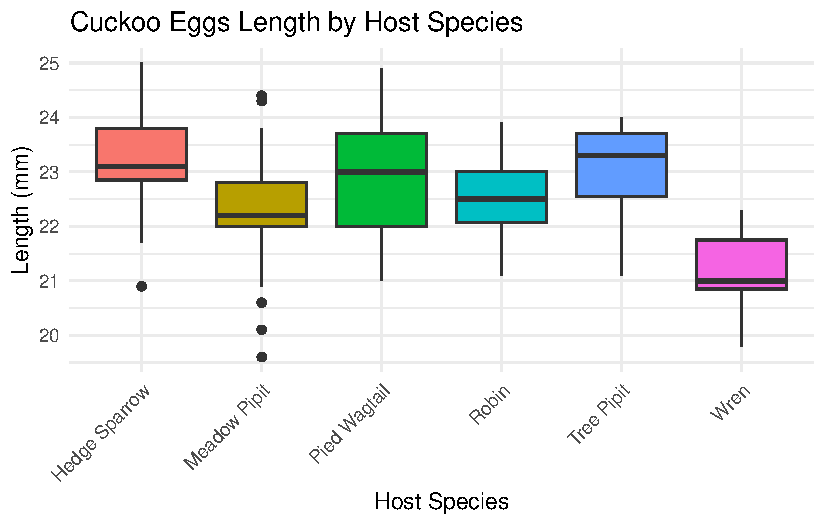
\includegraphics[keepaspectratio]{Capstone_project_files/figure-pdf/fig-boxplot-length-1.pdf}}

}

\caption{\label{fig-boxplot-length}Distribution of Cuckoo Egg Length by
Host Species}

\end{figure}%

\begin{figure}

\centering{

\pandocbounded{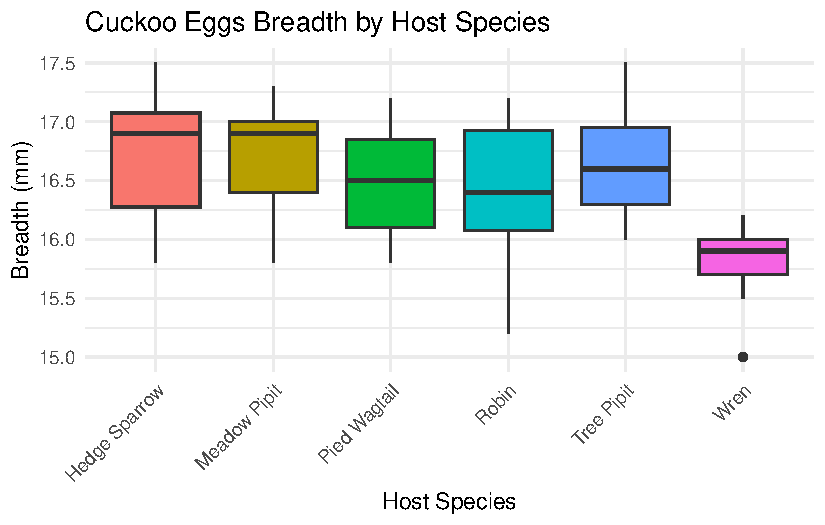
\includegraphics[keepaspectratio]{Capstone_project_files/figure-pdf/fig-boxplot-breadth-1.pdf}}

}

\caption{\label{fig-boxplot-breadth}Distribution of Cuckoo Egg Breadth
by Host Species}

\end{figure}%

\textbf{Observation}

\textbf{Length (Figure 1):} The boxplot for length shows clear
variations in egg size across species. The Tree Pipit displays the
highest median egg length (around 23.4 mm), closely followed by the
Hedge Sparrow (around 23.1 mm). The Pied Wagtail has a slightly lower
median but the largest interquartile range (the tallest box), indicating
a wider spread of egg lengths. In stark contrast, the Wren has the
distinctly lowest median length (around 21.0 mm). The Meadow Pipit shows
the most extreme variation, with a cluster of unusually small eggs (down
to 19.6 mm) and two unusually large outliers above 24 mm. The Hedge
Sparrow also has a single outlier egg at the lower end (exactly 20.9
mm).

\textbf{Breadth (Figure 2):} A similar pattern is visible in the
breadth. Hedge Sparrow and Meadow Pipit eggs are generally the widest
(highest medians, around 16.9 mm), while Wren eggs are the narrowest
(median around 16.0 mm). The Wren also has a single outlier egg with a
breadth of exactly 15.0 mm.

The visual separation in the medians and the spread of the boxes
strongly suggest that the host species influences the egg dimensions.
However, to prove that these differences are statistically significant
and not just due to random chance, inferential testing is required.

The visual separation in the medians and the spread of the boxes
strongly suggest that the host species influences the egg dimensions.
However, to prove that these differences are statistically significant
and not just due to random chance, inferential testing is required.

\subsection{Inferential Statistical
Analysis}\label{inferential-statistical-analysis}

To determine if the host bird species significantly influences the
physical dimensions of the eggs, a One-Way Analysis of Variance (ANOVA)
was performed. This test evaluates whether the means of the different
groups are statistically equal. A significance level of α=0.05 was used.

\textbf{1. ANOVA: Difference in Egg Length}

\textbf{- Null Hypothesis (Ho):} There is no significant difference in
the average length of eggs across the 6 bird species.

\textbf{- Alternative Hypothesis (H1):} At least one bird species has a
significantly different average egg length.

\begin{Shaded}
\begin{Highlighting}[]
\CommentTok{\# One{-}way ANOVA for Egg LENGTH by Species}
\NormalTok{length\_model }\OtherTok{\textless{}{-}} \FunctionTok{aov}\NormalTok{(length }\SpecialCharTok{\textasciitilde{}}\NormalTok{ species, }\AttributeTok{data =}\NormalTok{ cuckoo\_data)}
\FunctionTok{summary}\NormalTok{(length\_model)}
\end{Highlighting}
\end{Shaded}

\begin{verbatim}
             Df Sum Sq Mean Sq F value   Pr(>F)    
species       5  42.81   8.562   10.45 2.85e-08 ***
Residuals   114  93.41   0.819                     
---
Signif. codes:  0 '***' 0.001 '**' 0.01 '*' 0.05 '.' 0.1 ' ' 1
\end{verbatim}

\textbf{Result}

The ANOVA test yielded an F-statistic of 10.45 and a p-value of
2.85e-08. Because the p-value is significantly less than 0.05, we reject
the null hypothesis. This indicates that there is a highly statistically
significant difference in the length of cuckoo eggs depending on the
host bird species. The visual differences observed in the length boxplot
(Figure 1) are not due to random chance.

\textbf{2. ANOVA: Difference in Egg Breadth}

\textbf{- Null Hypothesis (Ho):} There is no significant difference in
the average breadth of eggs across the 6 bird species.

\textbf{- Alternative Hypothesis (H1):} At least one bird species has a
significantly different average egg breadth.

\begin{Shaded}
\begin{Highlighting}[]
\CommentTok{\# One{-}way ANOVA for Egg BREADTH by Species}
\NormalTok{breadth\_model }\OtherTok{\textless{}{-}} \FunctionTok{aov}\NormalTok{(breadth }\SpecialCharTok{\textasciitilde{}}\NormalTok{ species, }\AttributeTok{data =}\NormalTok{ cuckoo\_data)}
\FunctionTok{summary}\NormalTok{(breadth\_model)}
\end{Highlighting}
\end{Shaded}

\begin{verbatim}
             Df Sum Sq Mean Sq F value   Pr(>F)    
species       5  10.37  2.0746   10.88 1.41e-08 ***
Residuals   114  21.73  0.1906                     
---
Signif. codes:  0 '***' 0.001 '**' 0.01 '*' 0.05 '.' 0.1 ' ' 1
\end{verbatim}

\textbf{Result}

The ANOVA test yielded an F-statistic of 10.88 and a p-value of
1.41e-08. Because the p-value is significantly less than 0.05, we reject
the null hypothesis. This indicates that there is a highly statistically
significant difference in the breadth of cuckoo eggs depending on the
host bird species. The differences observed in the breadth boxplot
(Figure 2) are statistically valid.

\subsection{Conclusion}\label{conclusion}

This capstone project investigated whether the host bird species
influences the physical dimensions of cuckoo eggs. Through Exploratory
Data Analysis (EDA), it was observed that egg sizes vary visually across
the six species, with the Wren generally having the smallest eggs and
species like the Hedge Sparrow and Meadow Pipit having the largest. The
analysis also identified several outliers, particularly within the
Meadow Pipit species, indicating natural variance in egg sizes.

To mathematically test these visual observations, a One-Way Analysis of
Variance (ANOVA) was conducted for both egg length and breadth.

\begin{itemize}
\item
  For length, the ANOVA yielded a p-value of 2.85e-08.
\item
  For breadth, the ANOVA yielded a p-value of 1.41e-08.
\end{itemize}

Because both p-values are significantly lower than the 0.05 significance
level, we reject the null hypothesis. There is a highly statistically
significant difference in both the length and breadth of cuckoo eggs
depending on the host bird species.

These findings suggest that the cuckoo does not lay a uniform egg size
across all nests. Instead, the dimensions of the eggs vary significantly
by host species. This provides statistical evidence supporting the
evolutionary theory that brood parasites may adapt the physical
characteristics of their eggs to match the specific nest environment or
the size of the host bird, thereby maximizing the chances of the egg
being accepted and successfully incubated (Maindonald et al., 2015).

\subsection*{Reference}\label{reference}
\addcontentsline{toc}{subsection}{Reference}

\protect\phantomsection\label{refs}
\begin{CSLReferences}{1}{0}
\bibitem[\citeproctext]{ref-maindonald2015}
Maindonald, J. H., Braun, W. J., \& Braun, M. W. J. (2015). \emph{Cuckoo
eggs dataset (from the DAAG r package)}. Comprehensive R Archive Network
(CRAN). \url{https://CRAN.R-project.org/package=DAAG}

\end{CSLReferences}




\end{document}
